\documentclass[a4paper,12pt,openany]{book}
\usepackage [french]{babel}
\usepackage [utf8]{inputenc}
\usepackage [T1]{fontenc}
\usepackage{comment}
\usepackage{graphicx}
\usepackage{listings}
\usepackage{verbatim}
\usepackage{amsmath}
\usepackage{amsfonts}


%%configuration de listings
\lstset{
language=tex,
basicstyle=\ttfamily\small, 
identifierstyle=\color{red}, 
keywordstyle=\color{blue}, 
stringstyle=\color{black!60}, 
commentstyle=\it\color{green!95!yellow!1}, 
columns=flexible, 
tabsize=1, 
extendedchars=true, 
showspaces=false, 
showstringspaces=false, 
numbers=left, 
numberstyle=\tiny, 
breaklines=true, 
breakautoindent=true, 
captionpos=b
}

%coloration syntaxique
\usepackage{xcolor}
\definecolor{Zgris}{rgb}{0.87,0.85,0.85}

\author{Mendy Fatnassi}
\title{Cours Outils de Develloppement}

%%%%%%%%%%%%%%%%%%%%%%%%%%%%%%%%%%%%%%%%%%%%%%%%%%%%%%%%%%%%%%%%%%%%%%%%%%%%%%%%%%%%%%%%%%%%%%%%%%%%%%%%%%%%%%%%%
\begin{document}
\maketitle
\tableofcontents

\chapter{Latex}
Pour executer un document .tex via un terminal c-a-d en faire une version PDF , il suffit de taper \$pdflatex nom\_doc.tex \\
\\
\underline{Installer un package}:\\
T\'el\'echarger le .zip sur le site CTAN (librairie latex) puis copier les fichier du package dans le repertoire \/usr\/local\/share\/texmf\/tex\/latex
ensuite mettez a jour la liste des packages dans la base de donnée latex avec sudo texhash .\\
\\

\section{En-tete d'un document LaTeX}

\paragraph{}
Un document LaTeX commence par un en tete puis par le corps du document dans lequelle on vas ecire nos document .\\

\begin{verbatim}
\usepackage[latin1]{inputenc} % accents
\usepackage[T1]{fontenc}      % caractères français
\usepackage{geometry}         % marges
\usepackage[francais]{babel}  % langue
\usepackage{graphicx}         % images
\usepackage{verbatim}         % texte préformaté
\end{verbatim}

Ensuite on peux placer ces quelques commande pour reinseigner des information sur le document .\\

\begin{verbatim}
\title{Rapport de stage}      % renseigne le titre
\author{Prénom Nom}           %   "   "   l'auteur
\date{18 juin 2007}           %   "   "   la future date de parution
\pagestyle{headings}          % affiche un rappel discret (en haut à gauche)
                              % de la partie dans laquel on se situe
\end{verbatim}

Le corps du document seras delemité par des balises \verb+\begin{},\end{}+ , il faudra compiler le source LaTeX deux fois de suite pour qu'il gère correctement la table des matières :\\
Une première fois pour générer la table des matière et la seconde pour l'insérer dans le document.\\

\begin{verbatim}
\begin{document}
\maketitle				% genere le titre du document 
\tableofcontents		% genere la table des matieres 
...
\end{document}
\end{verbatim} 


\section{Des balises en Latex}

\subsection{Les caractere} \\
Les caract\`eres suivant sont utilis\'es par LaTeX pour la compilation (ils ont une signification particuli\`ere pour la mise en forme du texte) et ne peuvent donc figurer tels quels dans le texte : \\
\\
\verb+$ & % # { } _+ Il faudra les faire pr\'ec\'eder d'un "\textbackslash".\\
sauf pour :\\
\verb+« \ » 	qui s'écrit 	\textbackslash,+\\
\verb+« ~ » 	" 	\textasciitilde,+\\
\verb+« ^ » 	" 	\textasciicircum.+\\
\\
Pour les accents la syntaxe est la suivante : \ accent + lettre . 
Un accent peut etre aigue (\') ou grave (\`).\\
\underline{Exemple} : \'e (aigue) = \verb+é+\\
\\


\subsection{Mise en forme} \\
\\
\begin{DDbox}{\linewidth}
\begin{lstlisting}
	\underline %Souligne
	\textit ou \emph %italique
	\textbf %gras
\end{lstlisting}
\end{DDbox}{\linewidth}



\subsection{Inclure une image} \\

Inclure le package \verb+\usepackage{graphicx}+ et utiliser la balise : \\
\verb+\includegraphics[width=1\textwidth,center]{monimage.jpg}+\\
\\

\subsection{Tableaux}
On declare un tableau de la facons suivante : \\ 
\begin{verbatim}
\begin{center}
\begin{tabular}{|option|}
	\hline
	1 & 2 & 3 \\ \hline
	a & b & c \\ \hline
	4 & 5 & 6 \\ \hline
	\hline
\end{tabular}
\end{center}
\end{verbatim}
on obtient un tableau 3*3 avec comme option : l|c|r pour l'alignement de chacune des colonne .\\

\subsection{Les environnements}
-Pour afficher du code (C,HTML,...)}:
\begin{DDbox}{\linewidth}
\begin{lstlisting}
	\usepackage{listings}
	\begin{DDbox}{\linewidth}
	\begin{lstlisting}
	....Du texte....
	\end{lstlisting } 
	\end{DDbox}{\linewidth}
\end{lstlisting}
\end{DDbox}{\linewidth}


\section{Latex pour les Mathematiques}
\\
Inclure \verb+\usepackage{amsmath}+.Pour qu'un texte soit de la forme d'une expression math\'ematique on place le texte que l'on veux entre un bloc '\$\{text\}\$'.\\
\\
\subsection{Synthaxe} \\
\begin{verbatim}
\times = x (multiplication)
\div = symbole diviser
\ldots = ... (3 petits points)
\cdot = . (point centré , scalaire)
\overbrace{1,\ldots,n} = crochet du haut (ensemble)
\underbrace{1,\ldots,n} = crochet du bas (ensemble)
\neq =	≠ (difference)
\equiv = ≡ (equivalent)
\approx = ≈ (approximation)
\simeq = ≃ (approximation , plus au moins egal)
\leq, \geq = ≤ , ≥ 
\leqslant, \geqslant = ⩽ , ⩾ 
\ll, \gg = ≪ , ≫ 
\pm = ± 
\Rightarrow = ⇒ 
\Leftrightarrow = ⇔ 
\overline = barre au dessus (X barre)
\forall = ∀ (pour tous)
\exists = ∃	(existe)	
\emptyset = ∅ (vide)	
\in = ∈	(élément de)	
\notin = ∉	(pas un élément de)
\prod = ∏ (produit)	
\sum = ∑ (somme)	pour les indices \sum\limits_{i=0}^n
\wedge = ∧ (et)	
\vee = ∨ (ou)	
\cap = ∩ (point d'intersection)
\cup = ∪ (unité) 	
\subset = ⊂	(compris dans)
\notin = ⊄	(n'est pas compris dans)	
\end{verbatim}
\\

\subsection{Fonction Conditionnel }
\begin{verbatim}
\[
    f(x)= 
\begin{dcases}
    \frac{x^2-x}{x},& \text{if } x\geq 1\\
    0,              & \text{otherwise}
\end{dcases}
\]
\end{verbatim}\\

\underline{Les ensembles}:\\
il faut utiliser \verb+\usepackage{amsfonts}+ et la commande \verb+\mathbb{R}+ ce qui donne \mathbb{R}\\

\begin{verbatim}
La fonction $f$ est définie par
\[
   f(x) = x-1
\].
On a alors
\begin{equation}
   f(x) = 0 \iff x = 1
\end{equation}
\end{verbatim}
\\
\underline{Donne}:\\
\\
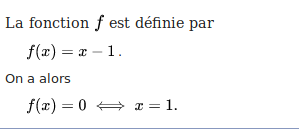
\includegraphics{latex_math_fonc.png}
\\
Liste de fonction pr\'ed\'efini :\\
\verb+\sin, \cos, \tan, \cot, \arcsin, \arccos, \arctan, \coth, \sinh, \cosh, \tanh, \ln, \log, \exp, \max, \min, \sup, \inf, \lim, \ker, \deg, \mod ;+\\
\\
Si l'on veut mettre du texte normal au sein de l'\'equation, il faut utiliser la fonction \verb+\text{texte}+ Si l'on veut mettre une lettre ou quelques lettres en romain, on utilise \verb+\mathrm{texte}+. De mani\`ere générale, les variables et les grandeurs physiques sont en italiques alors que les constantes « math\'ematiques » sont en romain.\\
\\
\subsection{Lettres Grecque} \\
Pour utiliser les lettres grecques, il suffit de taper leur nom en caractères latins pr\'ec\'ed\'e d'une contre-oblique.\\
\underline{Par exemple}:\\
\\
\verb+\alpha+ donne \alpha ;
\verb+\chi+ donne \chi ;
\verb+\omega+, \verb+\Omega+ donnent \omega, \Omega.
\verb+\epsilon+ donne \epsilon , \verb+\varepsilon+ donne \varepsilon ;
\verb+\theta+ donne \theta , \verb+\vartheta+ donne \vartheta ;
\verb+\pi+ donne \pi , \verb+\varpi+ donne \varpi ;
\verb+\rho+ donne \rho , \verb+\varrho+ donne \varrho ;
\verb+\sigma+ donne \sigma , \verb+\varsigma+ donne \varsigma ;
\verb+\phi+ donne \phi , \verb+\varphi+ donne \varphi ;
\\
\subsection{Exposant et Indices} \\
Pour mettre du texte en exposant, on le place dans un bloc et on le fait pr\'ec\'ecder d'un chapeau \verb+« ^ »+.\\
\\
Pour mettre du texte en indice, on place le texte dans un bloc et on le fait pr\'ec\'eder d'un tiret de soulignement \verb+« _ »+.\\
\\
L'opérateur somme (sigma majuscule S) s'écrit \verb+\sum+ ; pour écrire les limites de la somme, il suffit de les metre en indice et exposant :\\
\begin{verbatim}
    $\sum u_{n}$ ; $\sum_{i=1}^{n} (v_{i-1}+u_{i})$ 
    ou \sum\limits_{i=0}^n //si On veux que les indice soit placer en dessous de la somme
\end{verbatim}
\\
Donne : $\sum u_{n}$ ; $\sum_{i=1}^{n} (v_{i-1}+u_{i})$ \\
\\
\underline{par exemple}:\\
\begin{verbatim}
    $ u_n = 2^n $ donne un = 2n
    $ u_{n+1} = 2^{n+1} $ donne un+1 = 2n+1
\end{verbatim}

\subsection{Fraction \& Racines carré}\\
Une équation se place entre deux signes dollar « \$ ».\\
Pour écrire une fraction, nous utilisons la fonction 
\begin{verbatim}
\frac{dividende}{diviseur}
\end{verbatim}
\\
exemple : 
\begin{verbatim}
    $ \frac{a+b}{c-d} $ 
\end{verbatim}
\\
Pour mettre des grandes parenthèses, il faut mettre
\textbackslash left devant celle de gauche et 
\textbackslash right devant celle de droite :\\
\\
\begin{verbatim}
    $ \left( \frac{a+b}{c-d} \right)$ 
\end{verbatim}
\\
Pour les racines carré on utilise : \verb+\sqrt{}+\\
\\
\subsection{vecteur}
Vecteur : \\
\begin{verbatim}
\overrightarrow{AB}
ou
\vec{u}
\end{verbatim}
\\
Norme d'un vecteur :\\

\verb+\lVert levecteur \rVert+\\
ou ||u||\\

\subsection{limite de fonction}
La limite d'une fonction s'écrit de cette facons :\\
\verb!$\lim\limits_{x \rightarrow +\infty} f(x)$!\\
ce qui donne : $\lim\limits_{x \rightarrow +\infty} f(x)$ \\
et \\
\verb!$\lim\limits_{\subtrack{x \rightarrow -2 \\ x>-2}} f(x)$!\\
$\lim\limits_{\subtrack{x \rightarrow -2 \\ x>-2}} f(x)$\\

\subsection{Integrale}
Une integrale se note \verb+$\int_a^b f(x) \, \mathrm dt$+ .\\
$\int_a^b f(x) \, \mathrm dt$\\

\subsection{Matrice \& Vecteur Colonne}
On peux ecrire un vecteur colonne comme une matrice : \\
\begin{verbatim}
\begin{pmatrix}
a & b & c\\
d & e & f\\
g & h & i
\end{pmatrix}
\end{verbatim}\\
Ce qui donne : \\
\begin{pmatrix}
a & b & c\\
d & e & f\\
g & h & i
\end{pmatrix}

on peux utiliser \verb!\binom{n}{p}! pour superposer les 2 coeficients.\\

%%%%%%%%%%%%%%%%%%%%%%%%%%%%%%%%%%%%%%%%%%%%%%%%%%%%%%%%%%%%%%%%%%%%%%%%%%%%%%%%%%%%%%%%%%%%%%%%%%%%%%%%%%%%%%%%%%%%%%

\chapter{Debogage avec gdb}

Pour lancer l'option de debogage lors de la compilation d'un programme , il faut utiliser l'option -g de gcc , exemple : \\
\$gcc -g nom\_prog.c -o nom\_exec . Ensuite il faut lancer gdb , rien de plus simple : \$gdb nom\_exec .\\
\\
Voici quelque commande : \\
\\
\begin{center}
\begin{tabular}{|c|l|}
\hline
run/quit & Demarrer/Quitter \\ \hline
continue  & Reprendre l'execution \\ \hline
break num\_[ligne|fonction] | break nom_fic:nom\_[ligne|fonction] & Point d'arret \\ \hline
delete & Effacer tout les points d'arret \\ \hline
next|next nb\_ligne & Executer une (ou n) lignes pas a pas sans rentrer dans les sous-fonctions\\ \hline
step|step nb\_ligne & Executer une (ou n) lignes pas a pas en rentrant dans les sous-fonctions , dans les sources\\ \hline
finish & Execute jusqu'au retour de la fonction \\ \hline
print expr & Afficher la valeur de expression \\ \hline
up/down & Remonte/descend dans la pile d'appels \\ \hline
bt | bt full & affiche la pile d'appels \\ \hline

\end{tabular}
\end{center}

\underline{info breakpoints} : Affiche les point d'arret.\\
\\
\underline{watch} : On peux aussi introduire des watchpoint grace a la commande \textbf{watch {num\_ligne\|nom\_fonc}} , cela apour effet d'interompre l'execution du programme lorsque la valeur d'une variable a été modfié , on "surveille" la variable.\\
\\
\underline{backtrace} : Permet d'afficher la pile d'execution .\\
\\
\underline{where} : Affiche la pile des appels .\\
\\


%%%%%%%%%%%%%%%%%%%%%%%%%%%%%%%%%%%%%%%%%%%%%%%%%%%%%%%%%%%%%%%%%%%%%%%%%%%%%%%%%%%%%%%%%%%%%%%%%%%%%%%%%%%%%%%%%%%%%%

\chapter{Doxygen}

Doxygen parmet de creer de la documentation pour un code source , le fichier seras pars\'e par doxygen et creer la documentaion necessaire grace au commentaire inserer dans le code source .\\
\\
\$ doxygen -g nom_fichier --> Genere un fichier de configuration par defaut nomm\'e doxyfile. \\
\$ doxygen nom_doxy --> execute doxygen ,applique fichier de configuration doxygen sur les fichier commenter dans le repertoir du doxy .\\
\\

Pour commenter un code en doxygen on utiliseras les delimiteur suivant : \\
\begin{verbatim}
/**
*	\file nom_fic.c
*	\brief description
*	\author mendy
*/
\end{verbatim}
\\
Quelque balise : \\
\begin{verbatim}
\file <name>: Creer un bloc de documentation pour un fichier source ou d'en tete
\brief <description> : Permet d'ajouter une description 
\author <name> : Nom des auteurs 
\version <numeros> : Le numeros de la version du programme
\date <date> 

\fn <declaration fonction> : Permet d'ajoute un bloc de documentation pour une fonction , on peux detaille ca structure avec d'autre balise complementaire.
	\param <nom_param> : Descrit les parametre de la fonction
	\return <description_param> : descrit le parametre de retoure de la fonction

\struct <nom_struct> <nom_header_file> <nom_header> : Bloc de documentation pour une structure avec son nom , le nom de son header .h et un nom-optionnel pour le header . exemple : \struct Str_t str.h "definition" 
\end{verbatim}

%%%%%%%%%%%%%%%%%%%%%%%%%%%%%%%%%%%%%%%%%%%%%%%%%%%%%%%%%%%%%%%%%%%%%%%%%%%%%%%%%%%%%%%%%%%%%%%%%%%%%%%%%%%%%%%%%%%%%%

\chapter{github}

On commence avec un git init.\\
Pour indiqué que notre depot local pointe sur un depot distant : \\
git remote add OC https://github.com/OpenClassrooms-Student-Center/ProjetOpenSource.git \\
OC représente le nom court que vous utiliserez ensuite pour appeler votre dépôt.\\
\\
On se place dans un nouveau repertoire ou celui de notre choix puis on initialise un depot Git \textbf{\$git init} ensuite il faut y ajouter tous les fichier dans l'index de git \textbf{\$git add .}\\
Lorsqu'on modifie un repository, on doit enregistrer nos modifications dans Git en faisant un \textbf{\$git commit}.\\
L'option -m nous permet de lui envoyer un message decrivant les modifications effectuees.\\
\\
\textbf{\$git status} => Affiche les commits.\\
\textbf{\$git push } => Permet d'envoyez les modifications sur notre respository GitHub. \\
\textbf{\$git pull } => Permet de recuperer des modifications sur notre respository GitHub. \\
\textbf{\$git log } => Historique des commits.\\
\\
\textbf{\$git rm .} =>Quand on supprime des fichier, il reste dens l'indexe de fichier git pour cela on peux utiliser la commande "rm git ." pour validé la suppression des fichier apres un rm.
\\
\underline{Note}: L'expression "." et "*" sont differente. Exemple:\\
-\$git rm * supprime tout les fichier de l'indexe (\$git rm *.png -> supprime toute les image de type png).\\
-\$git rm . supprime uniquement les fichier de l'indexe marqué comme "supprimé".\\
\\
Git peux se parametrer grace a la commande \textbf{\$git config} .Cela permet de voir et modifier les variables de configuration qui contrôlent tous les aspects de l’apparence et du comportement de Git.\\
\\
Fichier /etc/gitconfig : Contient les valeurs pour tous les utilisateurs et tous les dépôts du système. Si vous passez l’option --system à git config, il lit et écrit ce fichier spécifiquement.\\
\\
Fichier ~/.gitconfig : Spécifique à votre utilisateur. Vous pouvez forcer Git à lire et écrire ce fichier en passant l’option --global.\\
\\
Fichier config dans le répertoire Git (c’est-à-dire .git/config) du dépôt en cours d’utilisation : spécifique au seul dépôt en cours.\\
\\
La première chose à faire après l’installation de Git est de renseigner votre nom et votre adresse de courriel. C’est une information importante car toutes les validations dans Git utilisent cette information.\\
\\
\begin{verbatim}
$ git config --global user.name "John Doe"
$ git config --global user.email johndoe@example.com
\end{verbatim}
\\
Pour verifier les parametres on peux utiliser la commande : \$\textbf{git config --list} \\
\\
-Gestion id et mp en memoire , il y a 3 mode : \\
\\
-Par défaut, rien n’est mis en cache. Toutes les connexions vous demanderont votre nom d’utilisateur et votre mot de passe.\\
\\
\underline{cache} : conserve en mémoire les identifiants pendant un certain temps.Par defaut le temps d'expiration est de 15min.\\
\\
\underline{store} : sauvegarde les identifiants dans un fichier texte simple sur le disque, et celui-ci n’expire jamais .\\
\\
\\
Vous pouvez choisir une de ces méthodes en paramétrant une valeur de configuration Git :\\
\\
\verb+$ git config --global credential.helper cache+\\
\\
Certains de ces assistants ont des options. \\
L’assistant  \textbf{store} accepte un argument --file <chemin> qui permet de personnaliser l’endroit où le fichier texte est sauvegardé (par défaut, c’est ~/.git-credentials).\\
\\
L’assistant cache accepte une option --timeout <secondes> qui modifie la période de maintien en mémoire.\\
\\
\underline{Exemple} :\\
\\
\verb+$ git config --global credential.helper 'store --file ~/.git-credentials'+\\
\\
Version moins securisé : \\
\begin{verbatim}
$git config --global user.name "your username"
$git config --global user.password "your password"
\end{verbatim}
\\
On peux aussi verifier dans les fichier \verb+~/.gitconfig et ~/.git-credentials+ si les information presente sont bien enregistré .\\

%%%%%%%%%%%%%%%%%%%%%%%%%%%%%%%%%%%%%%%%%%%%%%%%%%%%%%%%%%%%%%%%%%%%%%%%%%%%%%%%%%%%%%%%%%%%%%%%%%%%%%%%%%%%%%%%%%%%

\chapter{Compilation Makefile}
\\
Un Makefile peut être écrit à la main, ou généré automatiquement par un utilitaire (ex : automake,gmake etc). Il est constitué d’une ou de plusieurs règles de la forme :\\
\\
cible: dépendances\\
\\commandes
\\
Ce qui suit présente la création d’un Makefile pour un exemple de projet. Supposons pour commencer que ce projet regroupe trois fichiers exemple.h,exemple.c et main.c.\\
Un fichier Makefile de base de ce projet pourrait s’écrire :\\
\\
\underline{Exemple} : \\
\\
\begin{verbatim} 
mon_executable : exemple.o main.o
	gcc -o mon_executable exemple.o main.o

exemple.o: exemple.c
	gcc -o exemple.o -c exemple.c -Wall -O

main.o: main.c exemple.h
	gcc -o main.o -c main.c -Wall -O
\end{verbatim}
\\
On peux ameliorer notre makefile en rajoutant quelque cibles all: , clean: et mrproper: note Makefile devient donc : \\
\\
\underline{Exemple} : \\
\\
\begin{verbatim}
all: mon_executable

mon_executable: exemple.o main.o
	gcc -o mon_executable exemple.o main.o

exemple.o: exemple.c
	gcc -o exemple.o -c exemple.c -Wall -O

main.o: main.c exemple.h
	gcc -o main.o -c main.c -Wall -O

clean:
	rm -f *.o core
	
mrproper: clean
	rm -f mon_executable
\end{verbatim}
\\
Il est possible de définir des variables dans un Makefile. Elles se déclarent sous la forme NOM=valeur et sont appelées sous la forme \verb+$(NOM)+, à peu près comme dans un shellscript.Parmi quelques variables standards pour unMakefilede projet C ou C++, on trouve :\\
–CC : qui désigne le compilateur utilisé ;\\
–CFLAGS : qui regroupe les options de compilation ;\\
–LDFLAGS : qui regroupe les options d’édition de liens ;\\
–EXEC ou TARGET : qui regroupe les exécutables.\\
\\
\underline{Exemple}: \\
\\
\begin{verbatim}
CC=gcc
CFLAGS=-Wall -O
LDFLAGS=
EXEC=mon_executable

all: $(EXEC)

mon_executable: exemple.o main.o
	$(CC) -o mon_executable exemple.o main.o $(LDFLAGS)

exemple.o: exemple.c
	$(CC) -o exemple.o -c exemple.c $(CFLAGS)

main.o: main.c exemple.h
	$(CC) -o main.o -c main.c $(CFLAGS)

clean:
	rm -f *.o core
mrproper: clean
	rm -f $(EXEC)
\end{verbatim}
\\
Il existe aussi, et c’est encore plus intéressant car très puissant, des variables internes au Makefile, utilisables dans les commandes ; notamment :\\
\\
\begin{verbatim}
–$@+: nom de la cible ;
–$<: nom de la première dépendance ;
–$ˆ: liste des dépendances ;
–$?: liste des dépendances plus récentes que la cible ;
–$*: nom d’un fichier sans son suffixe;
\end{verbatim}
\\
\underline{Exemple} : \\
\\
\begin{verbatim}
CC=gcc
CFLAGS=-Wall -O
LDFLAGS=
EXEC=mon_executable

all: $(EXEC)

mon_executable: exemple.o main.o
	$(CC) -o $@ $^ $(LDFLAGS)

exemple.o: exemple.c
	$(CC) -o $@ -c $< $(CFLAGS)

main.o: main.c exemple.h
	$(CC) -o $@ -c $< $(CFLAGS)

clean:
	rm -f *.o core
mrproper: clean
	rm -f $(EXEC)
\end{verbatim}

\end{document}

%%%%%%%%%%%%%%%%%%%%%%%%%%%%%%%%%%%%%%%%%%%%%%%%%%%%%%%%%%%%%%%%%%%%%%%%%%%%%%%%%%%%%%%%%%%%%%%%%%%%%%%%%%%%%%%%%%%%

\chapter{Valgrind}

Valgrind est un debugueur qui permet de detcter les fuites de memoires dans un programme , en regardant le nombre de pointeur allouer et desallouer si ce nombre et different alors on auras des warnings pour nous expliquer les erreurs .\\
Pour lancer valgrind dans un terminale il suffit de taper \$valgrind ./nom_exec \\
\\
Il y a quelque section afficher dans le debugueur : \\
\\
\textbf{HEAP summary}:\\
Il s'agit d'un resumer de l'usage du tas car lorsqu'on utilise l'allocation dynamique ont alloue sur le tas .\\
\\
in use at exit : 0 bytes in 0 blocks \\
Cette ligne nous informe sur la quantite de memoire allouer dynamiquement et non liberee a la fin du programme .\\
\\
total heap usage : 0 allocs , 0 frees , 0 bytes allocated\\
Cette ligne informe de l'utilisation qui a ete faite de l'allocation dynamique . Le nombre d'allocation qui a ete faites , le nombres de liberation et la quantite total de memoire qui a ete demandee en tout au cours de l'execution du programme.\\
\\
Si on veux que valgrind nous affiche plus de detail on peux comppiler en mode debuge notre programme avec -g et utiliser les options --leak-check=full de valgrind \\
\\
\$gcc -g nom_prog.c -o nom_exec\\
\$valgrind --leak-check=full ./nom_exec\\
\\\